% chktex-file 2% chktex-file 29
% chktex-file 13
\documentclass[12pt]{report}
\usepackage{setspace}
\usepackage[a4paper, total={7in, 10in}]{geometry}
\usepackage[fleqn]{amsmath}
\usepackage{empheq}
\usepackage{amssymb}
\usepackage{amsthm}
\usepackage{gensymb}
\usepackage[fleqn]{cases}
\usepackage{multicol}
\usepackage{color}
\usepackage{stix}
\usepackage{chngcntr}
\usepackage{tikz}
\usepackage{enumitem}
\usepackage{pgfplots}
\usepackage{etoolbox}
\usepackage{tkz-euclide}
\usepackage{graphicx}
\usepackage{enumitem}
\usepackage{multirow}
\usepackage{mathtools}
\usepackage{mdframed}
\usepackage{adjustbox}
\usepackage{xpatch}
\usepackage{nicematrix}
\usepackage{ifthen}

\def\nswe#1#2#3{#1\,$#2^\circ\,#3'$}
\graphicspath{ {./assets/} }
\usetikzlibrary{calc,trees,positioning,arrows,fit,shapes,calc, decorations.markings}
\newcommand{\midarrow}{\tikz \draw[-triangle 90] (0,0) -- +(.1,0);}

\newcommand\typel[2]{
    \mathbin{\mathop{#1\kern0pt}%
        \limits_{\raisebox{3.6ex}{\hbox to0pt{\hss\strut$\uparrow$\hss}}\hbox to0pt{\hss#2\hss}}}
}

\newcommand\typem[2]{
    \mathbin{\mathop{#1\kern0pt}%
        \limits^{\raisebox{3.6ex}{\hbox to0pt{\hss#2\hss}}\hbox to0pt{\hss\strut$\downarrow$\hss}}}
}

\counterwithout{equation}{chapter}

\newcommand{\pgfplotsdrawaxis}{\pgfplots@draw@axis}
\newcommand\perm[2][^n]{\prescript{#1\mkern-2.5mu}{}P_{#2}}
\newcommand\permtwo[2][^n]{{}_{#1}P_{#2}}
\newcommand\comb[2][^n]{{}_{#1}C_{#2}}
\newcommand\combtwo[2][^n]{\prescript{#1\mkern-2.5mu}{}C_{#2}}
\makeatother
\pgfplotsset{only axis on top/.style={axis on top=false, after end axis/.code={
                    \pgfplotsset{axis line style=opaque, ticklabel style=opaque, tick style={thick,opaque},
                        grid=none}\pgfplotsdrawaxis}}}

\newtheorem{theorem}{Theorem}

\makeatletter
\xpatchcmd{\endmdframed}
{\aftergroup\endmdf@trivlist\color@endgroup}
{\endmdf@trivlist\color@endgroup\@doendpe}
{}{}
\makeatother

\mdfdefinestyle{MyFrame}{%
    linecolor=black,
    linewidth=1pt,
    roundcorner=20pt, innertopmargin=20pt,innerbottommargin=20pt, innerrightmargin=12pt,
    innerleftmargin=12pt, skipbelow=20pt, skipabove=20pt
    %backgroundcolor=gray!50!white}
}

\newcommand{\newitem}[1]{%
    \refstepcounter{subenum}%
    \parbox{\dimexpr.5\linewidth-.5\columnsep}{
        \makebox[\labelwidth][r]{(\thesubenum)\hspace*{\labelsep}} #1}\hfill }%%%

\setcounter{chapter}{21}

\setlength{\arrayrulewidth}{1pt}
\setlength{\tabcolsep}{12pt}

\begin{document}

\newcommand{\sol}[1]{

    \noindent \textbf{Sol.}
}
\newcommand{\prooff}[1]{

    \noindent \textbf{Proof.}
}

\newcommand{\sxrightarrow}[2][]{%
    \mathrel{\text{$\xrightarrow[#1]{#2}$}}%
}

\newenvironment{cequation}{
    \makeatletter
    \setbool{@fleqn}{false}
    \makeatother
    \begin{equation*}
        }{\end{equation*}}

\begin{titlepage}
    \raggedleft{}
    \rule{1pt}{\textheight}
    \hspace{0.02\textwidth}
    \parbox[b]{0.75\textwidth}{

    {\fontsize{40}{60}\selectfont\bfseries Mathematics}\\[2\baselineskip]
    {\huge\textit{Senior 3 Part I}}\\[4\baselineskip]
    {\Large\textsc{Melvin Chia}}

    \vspace{0.5\textheight}

    {\noindent Started on 10 April 2023}\\[\baselineskip]
    {\noindent Finished on XX XX 2023}\\[\baselineskip]
    {\noindent Actual time spent: XX days}\\[\baselineskip]}

\end{titlepage}

\chapter*{Introduction}
\addcontentsline{toc}{chapter}{Introduction} \markboth{INTRODUCTION}{}

\doublespacing{}
\section*{Why this book?}

\section*{Disclaimer}
\section*{Acknowledgements}

\singlespacing{}

\doublespacing{}
\tableofcontents
\singlespacing{}
\newpage

\setstretch{1.5}\subsection*{Exercise 22.1}

\begin{enumerate}
    \item Express the mapping from set $A$ to set $B$ using venn diagram, and determine
          which of the following mappings are functions.

          \begin{center}
              \begin{NiceTabular}{|c|c|c|c|}[cell-space-limits=8pt, corners, hvlines]
                  & Set $A$                                & Set $B$                                                                   & Mapping       \\
                  (a) & \{0, 3, 9, 12\}                        & \{0, 1, 2, 3\}                                                            & Divide by $3$ \\
                  (b) & \{-2, -1, 0, 1, 2\}                    & \{0, 1, 4, 9, 16\}                                                        & Power of $4$  \\
                  (c) & \{-2, -1, 0, 1, 2\}                    & \{0, 1, 4\}                                                               & Square        \\
                  (d) & \{30$^\circ$, 45$^\circ$, 60$^\circ$\} & $\left\{\dfrac{1}{2},\ \dfrac{\sqrt{2}}{2},\ \dfrac{\sqrt{3}}{2}\right\}$ & Sine          \\
                  (e) & \{-1, 0, 1, 2\}                        & \{-1, 0, 1\}                                                              & Cube          \\
              \end{NiceTabular}
          \end{center}

          \sol{}

          \setlength{\columnseprule}{1pt}
          \setlength{\columnsep}{24pt}

          \begin{multicols}{2}

              \begin{enumerate}[label=(\alph*)]
                  \item \adjustbox{valign=t}{
                            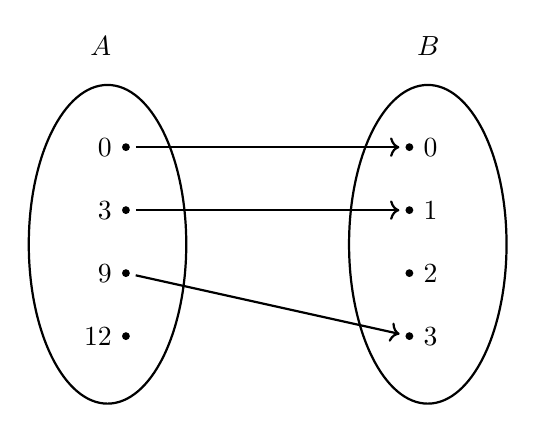
\begin{tikzpicture}[ele/.style={fill=black,circle,minimum width=.8pt,inner sep=1pt},every fit/.style={ellipse,draw,inner sep=4pt},scale=0.8]
                                \node[ele,label=left:$0$] (a1) at (0,4) {};
                                \node[ele,,label=left:$3$] (a2) at (0,3) {};
                                \node[ele,,label=left:$9$] (a3) at (0,2) {};
                                \node[ele,,label=left:$12$] (a4) at (0,1) {};
                                \node (a999) at (-0.5,1) {};

                                \node[ele,,label=right:$0$] (b1) at (4.5,4) {};
                                \node[ele,,label=right:$1$] (b2) at (4.5,3) {};
                                \node[ele,,label=right:$2$] (b3) at (4.5,2) {};
                                \node[ele,,label=right:$3$] (b4) at (4.5,1) {};
                                \node (b999) at (5,1) {};

                                \node[draw, thick,fit= (a1) (a2) (a3) (a4) (a999),minimum width=2cm] {} ;
                                \node[draw, thick,fit= (b1) (b2) (b3) (b4) (b999),minimum width=2cm] {} ;
                                \draw[->,thick,shorten <=2pt,shorten >=2] (a1) -- (b1);
                                \draw[->,thick,shorten <=2pt,shorten >=2] (a2) -- (b2);
                                \draw[->,thick,shorten <=2pt,shorten >=2] (a3) -- (b4);
                                \node at (-0.4,5.6) {$A$};
                                \node at (4.8,5.6) {$B$};
                            \end{tikzpicture}}
                        \vskip 0.5cm
                        Since $12 \in A$ has no image in $B$, this mapping is not a function.
                  \item \adjustbox{valign=t}{
                            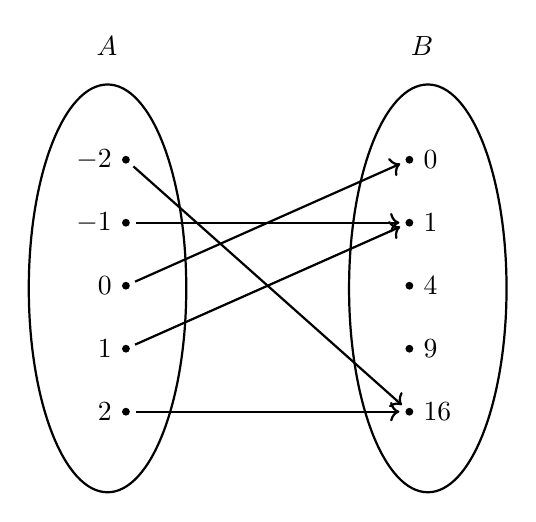
\begin{tikzpicture}[ele/.style={fill=black,circle,minimum width=.8pt,inner sep=1pt},every fit/.style={ellipse,draw,inner sep=4pt},scale=0.8]
                                \node[ele,label=left:$-2$] (a1) at (0,5) {};
                                \node[ele,,label=left:$-1$] (a2) at (0,4) {};
                                \node[ele,,label=left:$0$] (a3) at (0,3) {};
                                \node[ele,,label=left:$1$] (a4) at (0,2) {};
                                \node[ele,,label=left:$2$] (a5) at (0,1) {};
                                \node (a999) at (-0.5,1) {};

                                \node[ele,,label=right:$0$] (b1) at (4.5,5) {};
                                \node[ele,,label=right:$1$] (b2) at (4.5,4) {};
                                \node[ele,,label=right:$4$] (b3) at (4.5,3) {};
                                \node[ele,,label=right:$9$] (b4) at (4.5,2) {};
                                \node[ele,,label=right:$16$] (b5) at (4.5,1) {};
                                \node (b999) at (5,1) {};

                                \node[draw, thick,fit= (a1) (a2) (a3) (a4) (a5) (a999),minimum width=2cm] {} ;
                                \node[draw, thick,fit= (b1) (b2) (b3) (b4) (b5) (b999),minimum width=2cm] {} ;
                                \draw[->,thick,shorten <=2pt,shorten >=2] (a1) -- (b5);
                                \draw[->,thick,shorten <=2pt,shorten >=2] (a2) -- (b2);
                                \draw[->,thick,shorten <=2pt,shorten >=2] (a3) -- (b1);
                                \draw[->,thick,shorten <=2pt,shorten >=2] (a4) -- (b2);
                                \draw[->,thick,shorten <=2pt,shorten >=2] (a5) -- (b5);
                                \node at (-0.3,6.8) {$A$};
                                \node at (4.7,6.8) {$B$};
                            \end{tikzpicture}}

                        \vskip 0.5cm

                        Since each element in $A$ has an image in $B$, this mapping is a function.

                  \item \adjustbox{valign=t}{
                            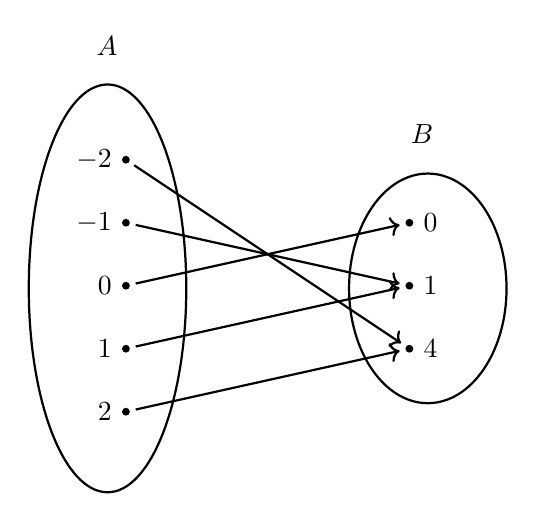
\begin{tikzpicture}[ele/.style={fill=black,circle,minimum width=.8pt,inner sep=1pt},every fit/.style={ellipse,draw,inner sep=4pt},scale=0.8]
                                \node[ele,label=left:$-2$] (a1) at (0,5) {};
                                \node[ele,,label=left:$-1$] (a2) at (0,4) {};
                                \node[ele,,label=left:$0$] (a3) at (0,3) {};
                                \node[ele,,label=left:$1$] (a4) at (0,2) {};
                                \node[ele,,label=left:$2$] (a5) at (0,1) {};
                                \node (a999) at (-0.5,1) {};

                                \node[ele,,label=right:$0$] (b1) at (4.5,4) {};
                                \node[ele,,label=right:$1$] (b2) at (4.5,3) {};
                                \node[ele,,label=right:$4$] (b3) at (4.5,2) {};
                                \node (b999) at (5,2) {};

                                \node[draw, thick,fit= (a1) (a2) (a3) (a4) (a5) (a999),minimum width=2cm] {} ;
                                \node[draw, thick,fit= (b1) (b2) (b3) (b999),minimum width=2cm] {} ;
                                \draw[->,thick,shorten <=2pt,shorten >=2] (a1) -- (b3);
                                \draw[->,thick,shorten <=2pt,shorten >=2] (a2) -- (b2);
                                \draw[->,thick,shorten <=2pt,shorten >=2] (a3) -- (b1);
                                \draw[->,thick,shorten <=2pt,shorten >=2] (a4) -- (b2);
                                \draw[->,thick,shorten <=2pt,shorten >=2] (a5) -- (b3);
                                \node at (-0.3,6.8) {$A$};
                                \node at (4.7,5.4) {$B$};
                            \end{tikzpicture}}

                        \vskip 0.5cm

                        Since each element in $A$ has an image in $B$, this mapping is a function.

                  \item \adjustbox{valign=t}{
                            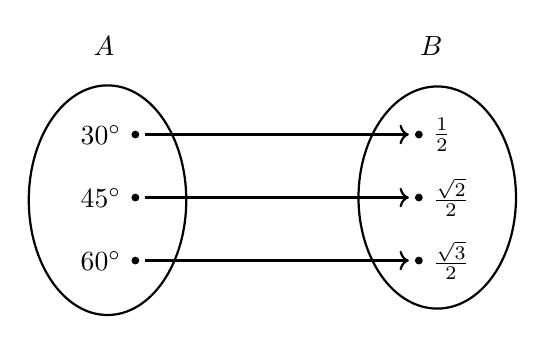
\begin{tikzpicture}[ele/.style={fill=black,circle,minimum width=.8pt,inner sep=1pt},every fit/.style={ellipse,draw,inner sep=4pt},scale=0.8]
                                \node[ele,label=left:$30^\circ$] (a1) at (0,3) {};
                                \node[ele,,label=left:$45^\circ$] (a2) at (0,2) {};
                                \node[ele,,label=left:$60^\circ$] (a3) at (0,1) {};
                                \node (a999) at (-0.8,1) {};

                                \node[ele,,label=right:$\frac{1}{2}$] (b1) at (4.5,3) {};
                                \node[ele,,label=right:$\frac{\sqrt{2}}{2}$] (b2) at (4.5,2) {};
                                \node[ele,,label=right:$\frac{\sqrt{3}}{2}$] (b3) at (4.5,1) {};
                                \node (b999) at (5,2) {};

                                \node[draw, thick,fit= (a1) (a2) (a3)  (a999),minimum width=2cm] {} ;
                                \node[draw, thick,fit= (b1) (b2) (b3) (b999),minimum width=2cm] {} ;
                                \draw[->,thick,shorten <=2pt,shorten >=2] (a1) -- (b1);
                                \draw[->,thick,shorten <=2pt,shorten >=2] (a2) -- (b2);
                                \draw[->,thick,shorten <=2pt,shorten >=2] (a3) -- (b3);
                                \node at (-0.5,4.4) {$A$};
                                \node at (4.7,4.4) {$B$};
                            \end{tikzpicture}}

                        \vskip 0.5cm

                        Since each element in $A$ has an image in $B$, this mapping is a function.

                  \item \adjustbox{valign=t}{
                            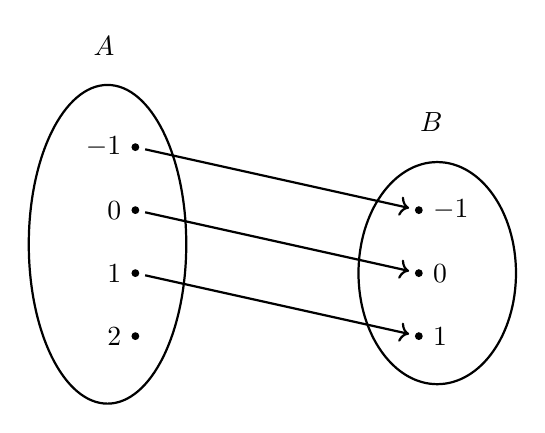
\begin{tikzpicture}[ele/.style={fill=black,circle,minimum width=.8pt,inner sep=1pt},every fit/.style={ellipse,draw,inner sep=4pt},scale=0.8]
                                \node[ele,label=left:$-1$] (a1) at (0,4) {};
                                \node[ele,,label=left:$0$] (a2) at (0,3) {};
                                \node[ele,,label=left:$1$] (a3) at (0,2) {};
                                \node[ele,,label=left:$2$] (a4) at (0,1) {};
                                \node (a999) at (-0.8,1) {};

                                \node[ele,,label=right:$-1$] (b1) at (4.5,3) {};
                                \node[ele,,label=right:$0$] (b2) at (4.5,2) {};
                                \node[ele,,label=right:$1$] (b3) at (4.5,1) {};
                                \node (b999) at (5,2) {};

                                \node[draw, thick,fit= (a1) (a2) (a3) (a4) (a999),minimum width=2cm] {} ;
                                \node[draw, thick,fit= (b1) (b2) (b3) (b999),minimum width=2cm] {} ;
                                \draw[->,thick,shorten <=2pt,shorten >=2] (a1) -- (b1);
                                \draw[->,thick,shorten <=2pt,shorten >=2] (a2) -- (b2);
                                \draw[->,thick,shorten <=2pt,shorten >=2] (a3) -- (b3);
                                \node at (-0.5,5.6) {$A$};
                                \node at (4.7,4.4) {$B$};
                            \end{tikzpicture}}

                        \vskip 0.5cm

                        Since $2 \in A$ does not have an image in $B$, this mapping is not a function.
              \end{enumerate}

          \end{multicols}

    \item Let function $f(x) = 3x^2 + 1$.

          \setlength{\columnseprule}{1pt}
          \setlength{\columnsep}{24pt}

          \begin{multicols}{2}
              \begin{enumerate}
                  \item Find the image of the following elements:
                        \begin{enumerate}
                            \item -3
                                  \sol{}
                                  \begin{flalign*}
                                      f(-3) & = 3(-3)^2 + 1 & \\
                                            & = 28
                                  \end{flalign*}

                            \item -2
                                  \sol{}
                                  \begin{flalign*}
                                      f(-2) & = 3(-2)^2 + 1 & \\
                                            & = 13
                                  \end{flalign*}

                            \item 0
                                  \sol{}
                                  \begin{flalign*}
                                      f(0) & = 3(0)^2 + 1 & \\
                                           & = 1
                                  \end{flalign*}

                            \item 2
                                  \sol{}
                                  \begin{flalign*}
                                      f(2) & = 3(2)^2 + 1 & \\
                                           & = 13
                                  \end{flalign*}

                            \item 5
                                  \sol{}
                                  \begin{flalign*}
                                      f(5) & = 3(5)^2 + 1 & \\
                                           & = 76
                                  \end{flalign*}
                        \end{enumerate}
                  \item Find the preimage of the following elements:

                        \begin{enumerate}
                            \item 13
                                  \sol{}
                                  \begin{flalign*}
                                      13 & = 3x^2 + 1 & \\
                                      12 & = 3x^2     & \\
                                      4  & = x^2      & \\
                                      x  & = \pm 2
                                  \end{flalign*}

                            \item 28
                                  \sol{}
                                  \begin{flalign*}
                                      28 & = 3x^2 + 1 & \\
                                      27 & = 3x^2     & \\
                                      9  & = x^2      & \\
                                      x  & = \pm 3
                                  \end{flalign*}
                            \item 1
                                  \sol{}
                                  \begin{flalign*}
                                      1 & = 3x^2 + 1 & \\
                                      0 & = 3x^2     & \\
                                      0 & = x^2      & \\
                                      x & = 0
                                  \end{flalign*}

                            \item 0
                                  \sol{}
                                  \begin{flalign*}
                                      0            & = 3x^2 + 1                & \\
                                      -1           & = 3x^2                    & \\
                                      -\frac{1}{3} & = x^2                     & \\
                                      x            & \text{ is not a real no.}
                                  \end{flalign*}

                            \item 4
                                  \sol{}
                                  \begin{flalign*}
                                      4 & = 3x^2 + 1 & \\
                                      3 & = 3x^2     & \\
                                      1 & = x^2      & \\
                                      x & = \pm 1
                                  \end{flalign*}
                                  \vspace{0.5cm}
                        \end{enumerate}
              \end{enumerate}
          \end{multicols}

    \item Let function $g(x) = 5x-2$. Find: \setlength{\columnseprule}{1pt}
          \setlength{\columnsep}{24pt}

          \begin{multicols*}{2}
              \begin{enumerate}
                  \item $g(-2)$
                        \sol{}
                        \begin{flalign*}
                            g(-2) & = 5(-2) - 2 & \\
                                  & = -12
                        \end{flalign*}

                  \item $g(-1)$
                        \sol{}
                        \begin{flalign*}
                            g(-1) & = 5(-1) - 2 & \\
                                  & = -7
                        \end{flalign*}

                        \vfill

                  \item $g(0)$
                        \sol{}
                        \begin{flalign*}
                            g(0) & = 5(0) - 2 & \\
                                 & = -2
                        \end{flalign*}
              \end{enumerate}
          \end{multicols*}

    \item Let function $f(x) = \left\{\begin{array}{ll}
                  \ \ \ \ \ \ 2x, & x \leq -1     \\
                  \ \ x-1,        & -1 \leq x < 3 \\
                  4x + 2,         & x \geq 3
              \end{array}\right.$, find

          \setlength{\columnseprule}{1pt}
          \setlength{\columnsep}{24pt}

          \begin{multicols}{2}

              \begin{enumerate}
                  \item $f(-5)$
                        \sol{}
                        \begin{flalign*}
                            f(-5) & = 2(-5) & \\
                                  & = -10
                        \end{flalign*}

                  \item $f(-2)$
                        \sol{}
                        \begin{flalign*}
                            f(-2) & = 2(-2) & \\
                                  & = -4
                        \end{flalign*}

                  \item $f(0)$
                        \sol{}
                        \begin{flalign*}
                            f(0) & = 0-1 & \\
                                 & = -1
                        \end{flalign*}

                        \vskip 20cm
                  \item $f(2)$
                        \sol{}
                        \begin{flalign*}
                            f(2) & = 2-1 & \\
                                 & = 1
                        \end{flalign*}

                  \item $f(10)$
                        \sol{}
                        \begin{flalign*}
                            f(10) & = 4(10) + 2 & \\
                                  & = 42
                        \end{flalign*}
              \end{enumerate}
          \end{multicols}

    \item Let $f: \mathbb{R} \to \mathbb{R}$, $f(x) = x^4$. Find the image of $-1$, 0, 1,
          and 2 under $f$. \sol{}
          \begin{flalign*}
              f(-1) & = (-1)^4 = 1 & \\
              f(0)  & = (0)^4 = 0  & \\
              f(1)  & = (1)^4 = 1  & \\
              f(2)  & = (2)^4 = 16
          \end{flalign*}

          \newpage

    \item Let $f: \mathbb{R} \to \mathbb{R}$, $f(x) = x^2$. Find the preimage of 0, 1,
          and 4 under $f$.

          In $\mathbb{R}$, which element does not have a preimage?

          \sol{}
          \vspace{-1.2cm}
          \setlength{\columnseprule}{0pt}
          \begin{multicols}{3}
              \begin{flalign*}
                  0 & = x^4 & \\
                  x & = 0
              \end{flalign*}

              \begin{flalign*}
                  1 & = x^4   & \\
                  x & = \pm 1
              \end{flalign*}

              \begin{flalign*}
                  4 & = x^4   & \\
                  x & = \pm 2
              \end{flalign*}
          \end{multicols}

          $\because\ \forall x \in \mathbb{R}$, $f(x) \geq 0$

          $\therefore$ $x \in \mathbb{R}^-$ does not have a preimage.

    \item In the diagram below, given that function $g: A \to B$ is defined as $g: x \to
              2x - 8$. Find the value of $a$ and $b$.
          \begin{center}
              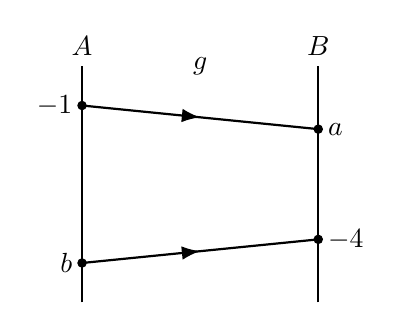
\begin{tikzpicture}
                  \draw[thick] (0,0) -- (0,3) node[above]{$A$};
                  \draw[thick] (3,0) -- (3,3) node[above]{$B$};
                  \node at (1.5, 3) {$g$};
                  \filldraw (0, 2.5) circle (1.5pt) node[left]{$-1$};
                  \filldraw (0, 0.5) circle (1.5pt) node[left]{$b$};
                  \filldraw (3, 0.8) circle (1.5pt) node[right]{$-4$};
                  \filldraw (3, 2.2) circle (1.5pt) node[right]{$a$};
                  \begin{scope}[thick,decoration={
                                  markings,
                                  mark=at position 0.5 with {\arrow{Latex}}}
                      ]
                      \draw[postaction={decorate}] (0, 2.5) -- (3, 2.2);
                      \draw[postaction={decorate}] (0, 0.5) -- (3, 0.8);
                  \end{scope}
              \end{tikzpicture}
          \end{center}
          \sol{}

          \begin{multicols}{2}
              \begin{flalign*}
                  a & = 2(-1) - 8 & \\
                    & = -10       & \\
              \end{flalign*}

              \begin{flalign*}
                  -4 & = 2b - 8 & \\
                  2b & = 4      & \\
                  b  & = 2
              \end{flalign*}
          \end{multicols}

    \item Using narrative form, arrow method, venn diagram, table method and graphical
          method, express the function $f(x) = 2x$, $x \in \{-2, -1, 0, 1, 2\}$.

          \sol{}

          \textbf{Narrative form:}

          Let $A = \big\{-2, -1, 0, 1, 2\big\}$ and $B = \big\{-4, -2, 0, 2, 4\big\}$,
          $f$ is a function from $A$ to $B$, its definition is that for any element $x$
          in $A$, its corresponding element is $2x$ in $B$.

          \newpage

          \textbf{Arrow method:}

          $f: -2 \to -4$, $-1 \to -2$, $0 \to 0$, $1 \to 2$, $2 \to 4$

          \textbf{Venn diagram:}
          \begin{center}
              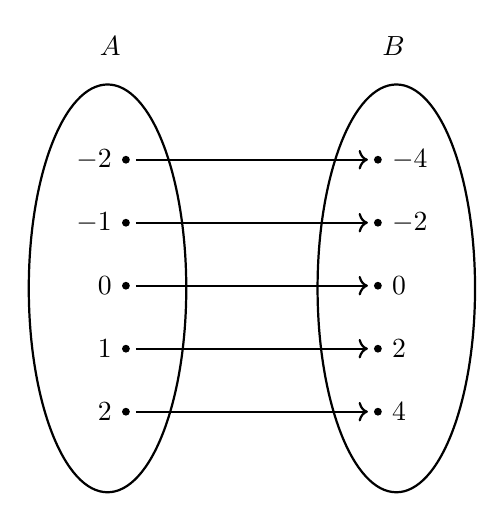
\begin{tikzpicture}[ele/.style={fill=black,circle,minimum width=.8pt,inner sep=1pt},every fit/.style={ellipse,draw,inner sep=4pt},scale=0.8]
                  \node[ele,label=left:$-2$] (a1) at (0,5) {};
                  \node[ele,label=left:$-1$] (a2) at (0,4) {};
                  \node[ele,label=left:$0$] (a3) at (0,3) {};
                  \node[ele,label=left:$1$] (a4) at (0,2) {};
                  \node[ele,label=left:$2$] (a5) at (0,1) {};
                  \node (a999) at (-0.5,1) {};

                  \node[ele,,label=right:$-4$] (b1) at (4,5) {};
                  \node[ele,,label=right:$-2$] (b2) at (4,4) {};
                  \node[ele,,label=right:$0$] (b3) at (4,3) {};
                  \node[ele,,label=right:$2$] (b4) at (4,2) {};
                  \node[ele,,label=right:$4$] (b5) at (4,1) {};

                  \node (b999) at (4.5,1) {};

                  \node[draw, thick,fit= (a1) (a2) (a3) (a4) (a5) (a999),minimum width=2cm] {} ;
                  \node[draw, thick,fit= (b1) (b2) (b3) (b4) (b5) (b999),minimum width=2cm] {} ;
                  \draw[->,thick,shorten <=2pt,shorten >=2] (a1) -- (b1);
                  \draw[->,thick,shorten <=2pt,shorten >=2] (a2) -- (b2);
                  \draw[->,thick,shorten <=2pt,shorten >=2] (a3) -- (b3);
                  \draw[->,thick,shorten <=2pt,shorten >=2] (a4) -- (b4);
                  \draw[->,thick,shorten <=2pt,shorten >=2] (a5) -- (b5);
                  \node at (-0.25,6.8) {$A$};
                  \node at (4.25,6.8) {$B$};
              \end{tikzpicture}
          \end{center}

          \textbf{Table method:}
          \begin{center}
              \begin{NiceTabular}{|c|c|c|c|c|c|}[code-before = \rectanglecolor{lightgray}{1-1}{2-1}, ]
                  \hline
                  $x$ & $-2$ & $-1$ & $0$ & $1$ & $2$ \\
                  \hline
                  $f(x)$ & $-4$ & $-2$ & $0$ & $2$ & $4$ \\
                  \hline
              \end{NiceTabular}
          \end{center}

          \textbf{Graphical method:}
          \begin{center}
              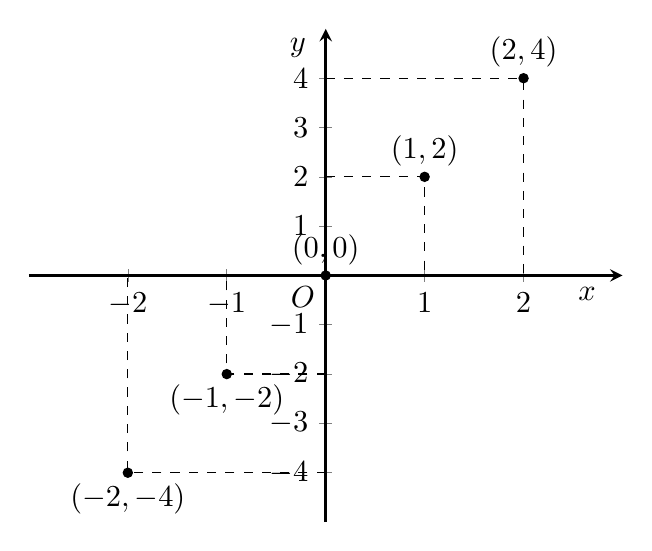
\begin{tikzpicture}[scale=1.1]
                  \begin{axis}[
                          axis lines = middle,
                          xlabel = $x$,
                          ylabel = {$y$},
                          ymin = -5,
                          ymax = 5,
                          xmin = -3,
                          xmax = 3,
                          xtick = {-2, -1, ..., 2},
                          ytick = {-4, -3, ..., 4},
                          xlabel style={below right, xshift=-1.8em, yshift=-0.05em},
                          ylabel style={above left, xshift=-0.3em, yshift=-1.3em},
                          axis line style={thick}
                      ]

                      \node at (axis cs:0,0) [anchor=north east] {$O$};

                      \filldraw[black] (axis cs:-2,-4) circle (1.5pt) node [below] {$(-2,-4)$};
                      \filldraw[black] (axis cs:-1,-2) circle (1.5pt) node [below] {$(-1,-2)$};
                      \filldraw[black] (axis cs:0,0) circle (1.5pt) node [above] {$(0,0)$};
                      \filldraw[black] (axis cs:1,2) circle (1.5pt) node [above] {$(1,2)$};
                      \filldraw[black] (axis cs:2,4) circle (1.5pt) node [above] {$(2,4)$};

                      \draw[dashed] (axis cs: 0, -4) -- (axis cs:-2,-4) -- (axis cs:-2,0);
                      \draw[dashed] (axis cs: 0, -2) -- (axis cs:-1,-2) -- (axis cs:-1,0);
                      \draw[dashed] (axis cs: 0, 0) -- (axis cs:0,0) -- (axis cs:0,0);
                      \draw[dashed] (axis cs: 0, 2) -- (axis cs:1,2) -- (axis cs:1,0);
                      \draw[dashed] (axis cs: 0, 4) -- (axis cs:2,4) -- (axis cs:2,0);
                  \end{axis}
              \end{tikzpicture}
          \end{center}
\end{enumerate}

\end{document}